\documentclass[12pt,a4paper]{article}
\usepackage[utf8]{inputenc}
\usepackage{amsmath}
\usepackage{amsfonts}
\usepackage{amssymb}
\usepackage[margin = 1in, bottom=1in, top=1in]{geometry}
\usepackage{fancyhdr}
\usepackage{graphicx}
\usepackage{titlesec}
\usepackage{float}
\usepackage{amsmath}
\usepackage[utf8]{inputenc}
\usepackage[english]{babel}
\usepackage{siunitx}
\usepackage{hyperref}
\usepackage[all]{hypcap}
\usepackage[export]{adjustbox}
\usepackage{textcomp}
\usepackage{gensymb}
\usepackage{physics}
\usepackage[nottoc,notlot,notlof]{tocbibind}
\newcommand\tab[1][1cm]{\hspace*{#1}}
\parindent 0ex
\titleformat{\subparagraph}
    {\normalfont\normalsize\bfseries}{\thesubparagraph}{1em}{}
\titlespacing*{\subparagraph}{\parindent}{3.25ex plus 1ex minus .2ex}{.75ex plus .1ex}
\usepackage[acronym,nomain]{glossaries}
\usepackage{slashbox}
\usepackage[acronym]{glossaries}




\titleformat{\paragraph}
{\normalfont\normalsize\bfseries}{\theparagraph}{1em}{}
\titlespacing*{\paragraph}
{0pt}{3.25ex plus 1ex minus .2ex}{1.5ex plus .2ex}
\setcounter{secnumdepth}{4}
\setcounter{tocdepth}{4}

\renewcommand{\headrulewidth}{0pt}


\fancypagestyle{a}{\fancyhf[L]{
\includegraphics[scale=0.30]{1.jpg}}\fancyhead[R]{
\includegraphics[scale=0.25]{2.jpg}}\fancyfoot[]}

\begin{document}

\begin{titlepage}
\begin{center}
\setcounter{page}{1}

\thispagestyle{a}
\vspace*{2cm}
\huge{\textbf{CIRCUIT DESIGN PROJECT}} \\[4mm]
\Large{\textbf{Hochschule Ravensburg - Weingarten}}\\ [1.5cm]

\line(1,0){450}\\
Morse Code Generator \\
\line(1,0){450}\\ [0.75cm]


 

\begin{tabbing}
\hspace{6cm}\=\hspace{4.5cm}\=\kill
 Project By: \> Noble Saji Pathil - 32374   \>  \\
  \> Lavanya Haridas - 33530 \>   \\ \\
 Guided By: \>Dr.-Ing., Professor Andreas Siggelkow  \>    \\ \\
 
   Submitted on:   \> 18.04.2022 \> 
\end{tabbing} 


\end{center}
\end{titlepage}

\newpage
\pagestyle{fancy}
\fancyfoot{}
\fancyhead{}

\setlength{\footskip=0pt}
\setlength{\headheight=35pt}

\newpage


\section*{Acknowledgement}

We are glad to express our indebtedness to our guide Prof. Dr. Andreas Siggelkow, Department of Electrical Engineering and Information Technology, Hochschule Ravensburg - Weingarten, for his valuable time and guidance, constant encouragement and kind help at various stages for the execution of the project task.\\

Also, Many students, especially my classmates and team member himself, have made valuable suggestions on this proposal which gave us an inspiration to improve our assignment. We are thankful to all the Students who help me in order to improve and execute our Assignment.\\

\newpage
\section*{Abstract}
In this project, we developed an implementation of Morse code generation in VHDL (Very High Speed Integrated Circuit Hardware Description Language). In this project, we used two FPGAs. One is responsible for the generation of the Morse-Code, from the message which is received from the PC. The other FPGA is responsible for receiving the message via Morse Code and is converted into ASCII code using Binary Search Algorithm. Once the message is acquired, it is transmitted by UART RS-232 protocol. This project requires two FPGAs- MAX1000 and hardware setup.We hvae designed out Circuitry to make computations as accurate as possible. We had to put our hard efforts to make it accurate so that for the large scale production of the chips executing this circuitry can be an optional design. \\


\newpage
\section*{Requirement and Objectives of the project}
The objective of this project is to learn how an engineer should design the Circuitry using VHDL programming, how things actually works in the real world. The ultimate target is to transmit the message from one point to other. From the PC, a C or C++ program needs to be written, which transmits the message from PC to the FPGA via UART receiver RS-232 protocol. Once the FPGA starts receiving the message via UART, one FPGA should be able to convert those characters in the message into Morse-Code. Once the FPGA generates the morse code signal, it is connected to an LED and start dispatching the characters through that LED. The speed should be 15 words per second. On the other side, another FPGA should be able to receive the morse encoded code via a Photo diode. Once, it receives the characters, it will convert it back in ASCII format and transmits it to another PC. On another PC, there is another C or C++ code which reads those ASCII characters and prints the message on the terminal. For testing, GTKterm has been used for the project.\\

There were certain requirement that has also been taken into consideration:
\begin{itemize}
\item The requirement is that the system should be able to transmit the message using morse code generation at 15 words per second.\

\item Finite State Machine algorithm has been used to prevent latches.

\item The whole block should have at least 4 signals: reset, clock, sensor signal, and txd signal.\

\item System clock speed is required to be 12MHz. \

\item The transmission should be using UART considering RS-232 protocol at 9K6 Hz.\
\end{itemize}

In the top level, it seems like that there are just two block that has been doing all the work. But actually, it works quite opposite. It has been divided into multiple small blocks that carries out small tasks and at the end, when all the blocks are connected, it seems like something big is happening. \\




\newpage
\pagestyle{fancy}
\fancyfoot{}
\fancyhead{}
\setlength{\footskip=25pt}
\setlength{\headheight=0pt}
%\renewcommand{\footrulewidth}{0.4pt}

\fancyfoot{}
\newpage

\rfoot{Page $\vert$ \thepage}
\pagenumbering{roman}
\setcounter{page}{5}
\tableofcontents
\clearpage

\section*{Section with acronyms}



\newacronym{gcd}{GCD}{Greatest Common Divisor}
\newacronym{lcm}{LCM}{Least Common Multiple}
\printglossary[type=\acronymtype]


\addcontentsline{toc}{section}{\listfigurename}
\listoffigures
\clearpage


\fancyfoot{}
\rfoot{\thepage}
\pagenumbering{arabic}
\setcounter{page}{1}
\renewcommand{\baselinestretch}{1.5} % line space
\section{Introduction}
There are certain arrangements needed in order to do the design of this Circuitry, such as the Hardware Setup, Software Setup for Simulation and Software to upload the code to the FPGA boards. These things are going to be discussed in this Chapter. In order to upload the code into the FPGA board, a short description is required for the FPGA.\

%\thispagestyle{c}
\subsection{Introduction to FPGA }
A Field Programmable Gate Array (FPGA) is a semiconductor device containing programmable logic components and programmable interconnects. The programmable logic components can be programmed to duplicate the functionality of basic logic gates such as AND, OR, NOT, XOR or more complex combinational functions such as decoders or math functions. The FPGA configuration is generally specified using a hardware description language (HDL). The most common FPGA architecture consists of an array of logic blocks called Configurable Logic Block (CLB) or Logic Array Block (LAB), I/O pads- to make off chip connections and programmable routing channels to implement logical functions. FPGAs have analogue features in addition to digital functions. The most common analogue feature is programmable slew rate and drive strength on each output pin. Another relatively common analogue feature is differential comparators on input pins designed to be connected to differential signalling channels.\\


\subsection{Introduction to the hardware used for the Project}
The MAX1000 FPGA development Board provides all the basic features and said to logically optimized.
\begin{itemize}

\item For applications where logic densities matters more than I/O count.\
\item Ideal for logic integration, DSP co-processing and embedded control, requiring significant processing and narrow or few interfaces.
\end{itemize}

For the project, MAX1000 FPGA development board is used. The MAX1000 FPGA board comes built in with many peripherals that help in the proper working of the board and also in interfacing the various signals to the board itself. It has dual flash inside, ADC with 8x12Bits, temperature range of 0...85°C, supply through USB pin, on-board USB programmer, MEMS Oscillator of 12 MHz. \\

Moreover, it has about 8000 Logic gates and has 1 Msps 12 bit ADC for analogue signals and 3.3V power supply. Some more features includes embedded SRAM, DSP blocks, instant-on within milliseconds and the abality to implement intel soft core embedded processor to perform microcontroller tasks. \\

\subsection{Information about VHDL}
VHDL(VHSIC-Very High Speed Integrated Circuit  Hardware Description Language)  is a hardware description language used in electronic design automation to describe digital and mixed-signal systems such as field-programmable gate arrays and integrated circuits. VHDL can also be used as a general purpose parallel programming language.
VHDL is commonly used to write text models that describe a logic circuit. Such a model is processed by a synthesis program, only if it is part of the logic design. A simulation program is used to test the logic design using simulation models to represent the logic circuits that interface to the design. This collection of simulation models is commonly called a testbench.\\
A VHDL simulator is typically an event-driven simulator. This means that each transaction is added to an event queue for a specific scheduled time. E.g. if a signal assignment should occur after 1 nanosecond, the event is added to the queue for time +1ns. Zero delay is also allowed, but still needs to be scheduled: for these cases Delta delay is used, which represent an infinitely small time step. The simulation alters between two modes: statement execution, where triggered statements are evaluated, and event processing, where events in the queue are processed.\\
VHDL has constructs to handle the parallelism inherent in hardware designs, but these constructs (processes) differ in syntax from the parallel constructs in Ada (tasks). Like Ada, VHDL is strongly typed and is not case sensitive. In order to directly represent operations which are common in hardware, there are many features of VHDL which are not found in Ada, such as an extended set of Boolean operators including NAND and NOR.\\
VHDL has file input and output capabilities, and can be used as a general-purpose language for text processing, but files are more commonly used by a simulation testbench for stimulus or verification data. There are some VHDL compilers which build executable binaries. In this case, it might be possible to use VHDL to write a testbench to verify the functionality of the design using files on the host computer to define stimuli, to interact with the user, and to compare results with those expected. However, most designers leave this job to the simulator.\\
It is relatively easy for an inexperienced developer to produce code that simulates successfully but that cannot be synthesized into a real device, or is too large to be practical. One particular pitfall is the accidental production of transparent latches rather than D-type flip-flops as storage elements.\\
One can design hardware in a VHDL IDE (for FPGA implementation such as Xilinx ISE, Altera Quartus, Synopsys Synplify or Mentor Graphics HDL Designer) to produce the RTL schematic of the desired circuit. After that, the generated schematic can be verified using simulation software which shows the waveforms of inputs and outputs of the circuit after generating the appropriate testbench. To generate an appropriate testbench for a particular circuit or VHDL code, the inputs have to be defined correctly. For example, for clock input, a loop process or an iterative statement is required$[12]$\\
A final point is that when a VHDL model is translated into the "gates and wires" that are mapped onto a programmable logic device such as a CPLD or FPGA, and then it is the actual hardware being configured, rather than the VHDL code being "executed" as if on some form of a processor chip.\\



\newpage

\renewcommand{\baselinestretch}{1.5} % line space
\section{GUIDELINES AND REQUIREMENT}
Everything related to circuit designing with VHDL will be discussed in this Chapter. This chapter includes the design guidelines that has to be done while programming with VHDL. These guidelines are ideal and are currently used worldwide. This chapter also describes the requirements that need to be fulfilled.\\

\subsection{Design Guidelines}
There are certain guidelines that need to follow:\\

\begin{enumerate}


\item A filename or dirname MUST NOT start with a special char or a number. \
\item A dot MUST BE used as a separator between filename and its extension.\\
	Example :     \hspace{1cm} content of the file has to be\\
	mycirc\_e.vhd \hspace{1cm} a VHDL-entity called mycirc\_e\\
	mycirc\_a.vhd \hspace{1cm} a VHDL-entity called mycirc\_a or mycirc\_a1\\
	README.txt    \hspace{1cm} some text\\

\item VHDL directories should be in the Tree Structure. This tree structures of four more directories inside(Documentation, Presentation, gcc and VHDL). The documentation directory consists of a report.pdf file(file name can be anything). The Presentation directory should consist a presentation.ppt or .pptx (filename can be anything). The gcc directory consists of the C-code that reads the data coming from the port ttyS0. The VHDL code should have the three more directories, sim – it consists of the simulation work file used in ModelSim to stimulating the code; src – it consists of the all the files related to VHDL program with the top level file.\

\item In source files, Each ENTITY has its own file. Each ARCHITECTURE has its own file. And each Architecture has its own TESTBENCH(es).\
\item Use of TABS is forbidden.\
\item Using more than 80 characters per line is forbidden.\ 
\item For signal-names in entities, the following rule should be applied:\
\begin{itemize}
\item rb\_i \hspace{1cm} 	: input, async. Global reset, active low\
\item cp\_i \hspace{1cm}  	: input, async. Global System clock, active at rising edge \
\item xx\_i \hspace{1cm}  	: input signal named xx\_i\
\item xx\_o \hspace{1cm}    : output signal named xx\_o\
\item xy\_io\hspace{1cm} 	: in-out signal\
\end{itemize}

\item For all signals in Architecture, rules are : xyz\_s  : an internal signal named xyz\_s\
\item All architectures containing memory must have an input called rb\_i and cp\_i.\
\item All architecture containing no memory must not have an input called rb\_i  and cp\_i.\
\item Constants and components must be defined in a Package\


\end{enumerate}


\subsection{Requirements}
There are certain requirements that need to be fulfilled. This requirement section basically consists of Hardware requirements and software requirements.\\

The Hardware requirements includes :\
\begin{itemize}
\item A two PC-FPGA set up for morse code conversation and message transmission.\
\item A photo diode to be connected on the reception FPGA\
\item DB9 RS-232 Cables from FPGA board to PC and vice versa\
\item System Clock and Asynchronous Reset button\
\item Two MAX1000 FPGA board for circuits implementation\
\item UART for data transmission to PC\
\item PC with UART interface\
\end{itemize}

The Software requirements includes :\
\begin{itemize}
\item VHDL for Programming FPGA and UART\
\item C-code for printing the data coming from the port ttyS0 or ttyS1 at the baudrate 9600 Hz\
\item MODELSIM or System Simulation\
\item ISE for synthesizing the VHDL program and uploading to the FGPA board\
\end{itemize}

\newpage
\renewcommand{\baselinestretch}{1.5} % line space
\section{History / Revision / Change Management}

This chapter consists of the changes and revision done through out the project. \\

\begin{center}
\begin{tabular}{ | c | c| c | } 
  \hline
  \textbf{Version no.}& \textbf{Comment} & \textbf{Date} \\ 
  \hline
  0.1 & First Draft of Specification & 18.04.2022 \\ 
  \hline
\end{tabular}
\end{center}


\newpage

\renewcommand{\baselinestretch}{1.5} % line space
\section{CIRCUIT DESIGNING WITH VHDL}
A brief overview of the top level of the Circuit blocks will be described in this chapter. Moreover, the top level consists of some small blocks such as Counters, multiplexers,etc is going to described in this chapter.\\


\subsection{Top Level Block Diagram Entity}

\begin{figure}[H]
\centering
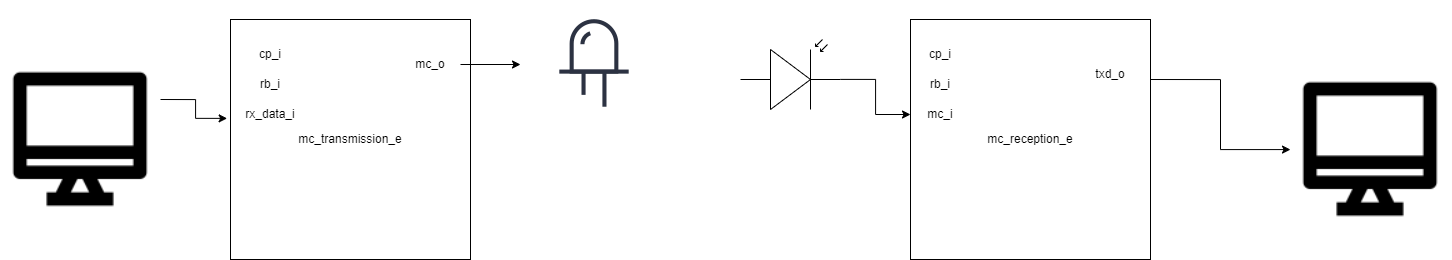
\includegraphics[scale=0.25]{top.drawio.png}
\caption{Top Level Entity}
\label{Top Level Entity}
\end{figure}


\begin{enumerate}
\item \textbf{cp\_i:} cp\_i denotes the system clock. It is a contineous sequence of low and High on the line providing to it. The system clock is needed to synchronize all the components that is running on the FPGA board. That means, they all do their work only if the clock is high;never when it’s low. And because of the clock speed is set above the longest time any signal needs to propogatethrough any circuit on the board,this signals is preventing signals from arriving before other signals and thus makes everything safe and synchronyzed.

\item \textbf{rb\_i:} rb\_i denotes the reset button signal. It is an active low signal. It is a signal that initialize the complete system. Reset can be switch button or a push button and is generally used by the user. It restart all the interfaces and all the State Machines which are working inside the FPGA chip, are forced to go to its initial state. 

\item \textbf{rx\_data\_i:} rx\_data\_i is the signal that is coming from the PC, that is placed on the FPGA Set up. This signal is responsible for transmitting the message characters to the FPGA via ASCII.

\item \textbf{mc\_o:} mc\o signal is the signal which is being forwarded to the LED, which represents the Morse code transmission via the dot and dash blinking of the LED.

\item \textbf{mc\_i:} mc\_i signal is the signal which represent the morse encoded signal and is taken as an input in the another FPGA.

\item \textbf{txd\_o:} txd\_o signal is the signal which represent the transmission of the Morse to ASCII converted data.

\item There were also some other signals that has been taken out, just for testing purpose.
\end{enumerate}

\begin{figure}[H]
\centering
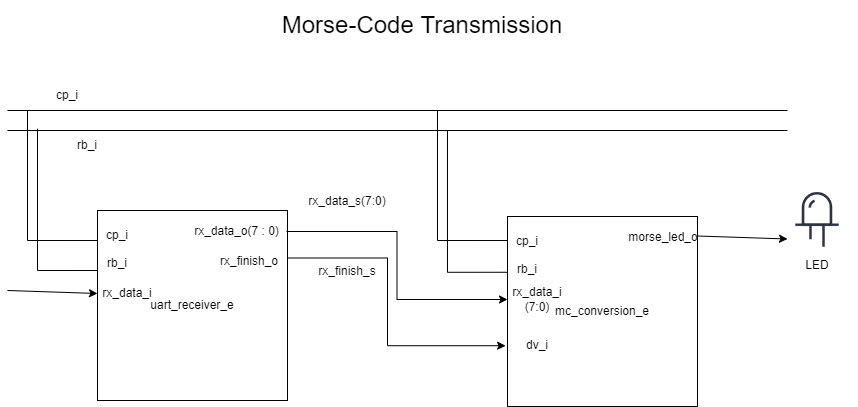
\includegraphics[scale=0.5]{MC_transmission.drawio.png}
\caption{Morse Code Transmission Architecture}
\label{Top Level Architecture}
\end{figure}

\begin{figure}[H]
\centering
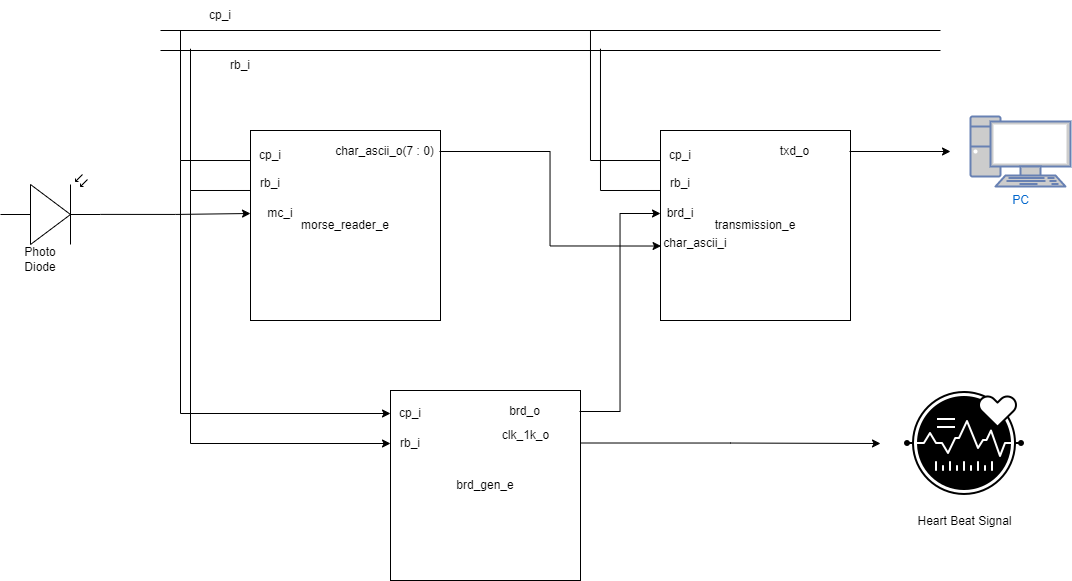
\includegraphics[scale=0.45]{MC_reception.drawio.png}
\caption{Morse Code Reception Architecture}
\label{Top Level Architecture}
\end{figure}
\newpage



\subsection{Top level block diagram Architecture}
As it can be seen, the top level architecture is a divided into two parts and it is very hard to understand everything at a single glance. Basically, it provides an architecture where a message is sent from one place to another using the Morse code generator. \

As it becomes a bit complicated to understand, let’s try to break it down into small modules. The very first module is uart\_receiver\_e which received the recipient data, which is coming from the PC serially, is being received into a 8-bit data representing a character in ASCII and a finish signal representing that the 8-bit data is received and signals the following component to start the computation.\
 
The next module is mc\_conversion\_e block. This is bascially responsible for converting the ASCII received data into Morse-Code and this signal is forwarded to the LED through which the morse encoded worded is transmitted.\

The next module is morse\_reader\_e block. This is implemented on the recipient side of the system. The signal from the photo diode is forwarded to this component. This component reads the morse code and converts it into ASCII word representing the character and is forwarded to the following component.\

The next block is the brd\_gen\_e block. This block keeps on generating the brd\_o which is the 9K6 baud rate signal. It also generates the one second signal which represents the heart beat signal for the FPGA.

The last remaining is the Transmission\_e (UART) block. It is responsible for sending the ASCII data that is coming from the morse\_reader\_e serially through a single signal. That is the output of the top level architecture and is connected to the computer.
\begin{figure}[H]
\centering
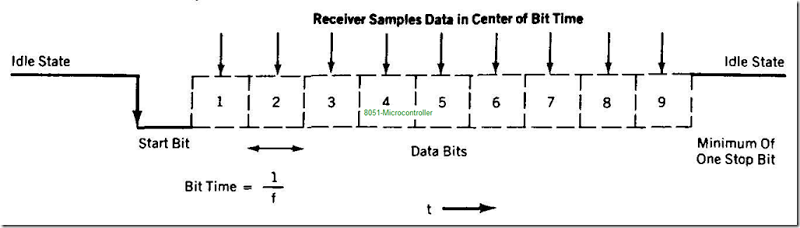
\includegraphics[width=\linewidth]{urattime.png}
\caption{The UART bit sequence }
\label{the UART bit sequence }
\end{figure}

So far, the overview of the top level architecture is explained. The detailed description of each block is given in the following sections.\

\subsection{uart\_receiver\_e}
The entity of the uart\_receiver\_e looks like :\\

\begin{figure}[H]
\centering
\includegraphics[scale=1.0]{uart\_receiver\_e.png}
\caption{UART Receiver Entity}
\label{UART Receiver Entity}
\end{figure}

As mentioned above, this block is implemented for receiving the message using UART protocol from the PC. This is an Synchronous block and has asynchronous reset signal which resets the whole block. The output of this block gives out two signals, rx\_data\_o which passes 8 bit ASCII data of the characters in the message and rx\_finish\_o, which shows that the reception is finished and the data is valid. 


\subsection{mc\_conversion\_e}
The mc\_conversion\_e is a block which converts the ASCII character of 8 bit into morse code and is transmitted to the LED. This is done using Logic table and a bunch of multiplexers. Using the logic table, the ASCII character is translated to Morse encoded code and clears the necessary signals if needed. \\

\begin{figure}[H]
\centering
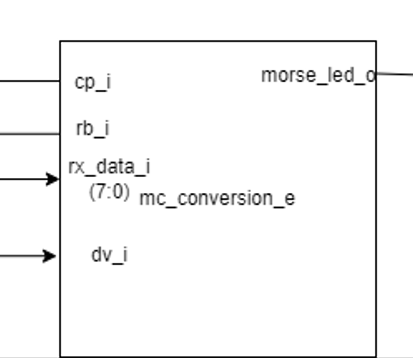
\includegraphics[scale=1.0]{mc_conversion_e.PNG}
\caption{ An Entity of the Morse Code Conversion block}
\label{An Entity of the Morse Code Conversion block}
\end{figure}


\subsection{morse\_reader\_e}
The morse\_reader\_e block is responsible for reading the signals or dot and dashes which is coming from the photo diode and is converted into the ASCII character.\\

This is how the architecture of the morse\_reader\_e looks like :\\
\begin{figure}[H]
\centering
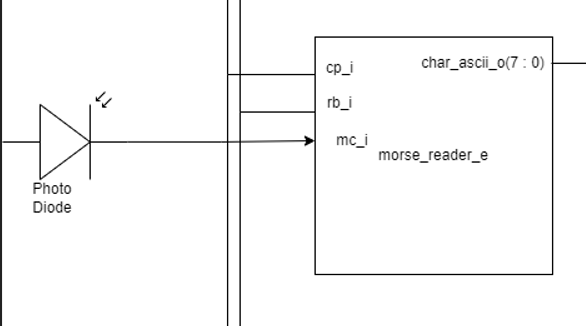
\includegraphics[scale=1.0]{morse_reader_e.PNG}
\caption{Entity of the Morse Reader Entity}
\label{Entity of the Morse Reader Entity}
\end{figure}

The conversion of Morse code to ASCII characters is done using Binary Search Tree Algorithm. This follows a tree like structure and deducts the ASCII characters. \\

\begin{figure}[H]
\centering
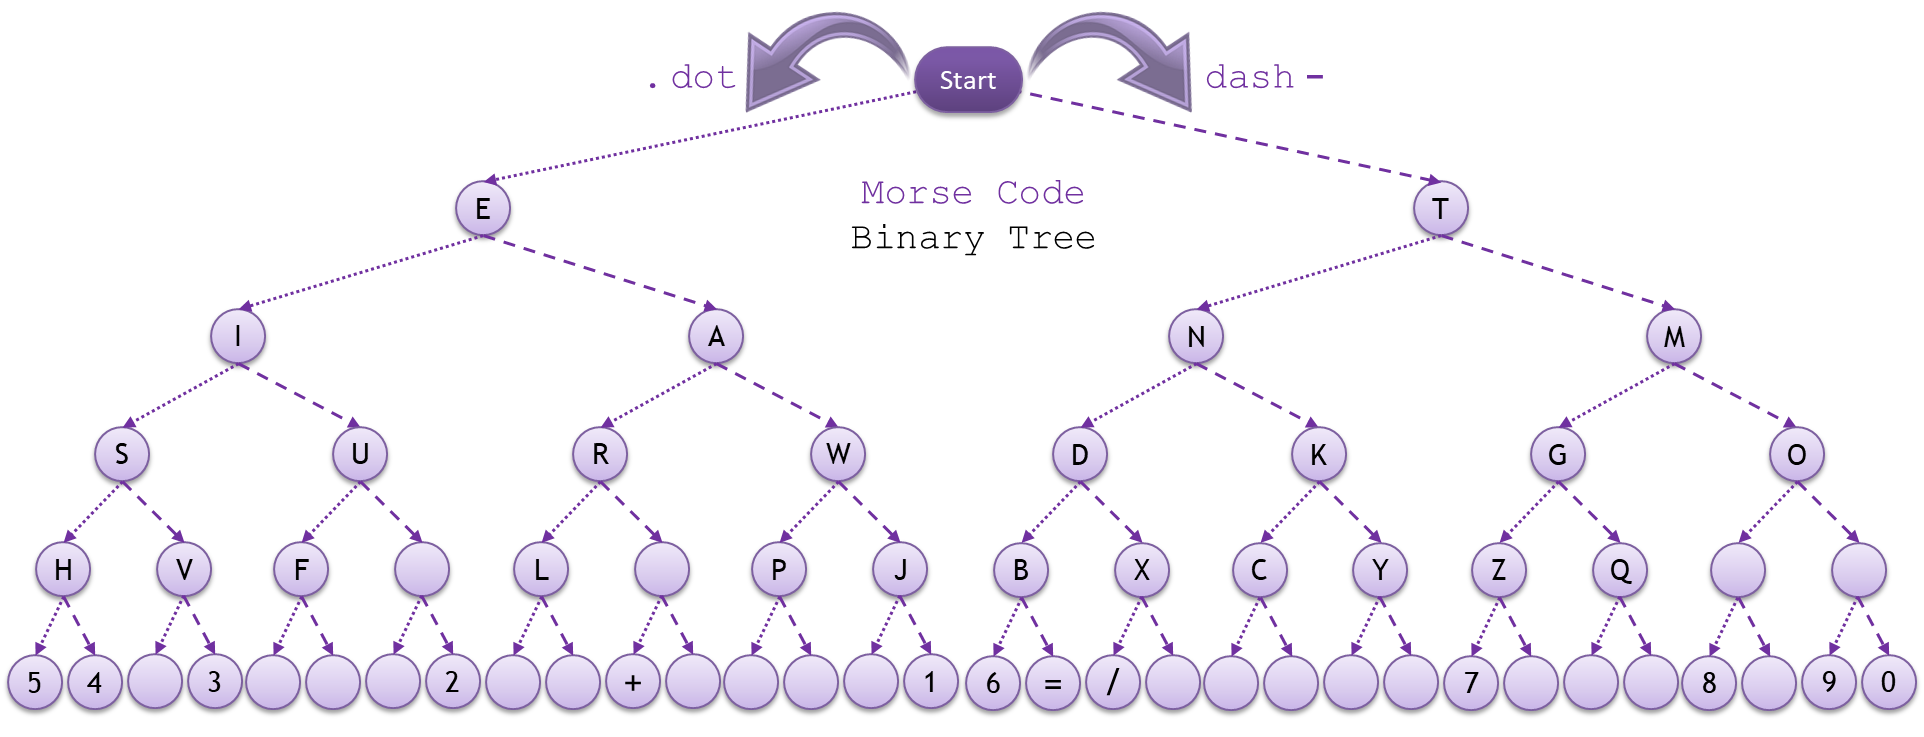
\includegraphics[scale=0.5]{bst.png}
\caption{architecture of the Binary Search Tree Algorithm}
\label{architecture of the Binary Search Tree Algorithm}
\end{figure}


\subsection{brd\_gen\_e}
This block is responsible for generating the 9600 Hz Baud rate signal. It also generates the one second signal which represents for the heart beat of the system.\\ 

The entity seems to be like :\\
\begin{figure}[H]
\centering
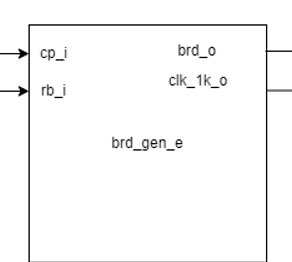
\includegraphics[scale=1.0]{brd_gen_e.PNG}
\caption{Entity of the Baud rate generator}
\label{Entity of the Baud Rate Generator}
\end{figure}

\subsection{Transmission (UART)}
As mentioned above, this block is responsible for transmitting the data to the computer. UART is a device that has the capabilities to both receive and transmit data. UART exchanges text data into American Standard Code For Information Interchange(ASCII)  format. In that, each alphabetical character is encoded by 7-bits and transmitted as 8 data bits. The transfer of the ASCII pattern is being done inside the transmission block(UART). For the transmission, the UART protocol wraps this 8-bit sub word with a start bit in the least significant bit and a stop bit in the most significant bit. The diagram shown below shows a lot of things about the UART:\\


\begin{figure}[H]
\centering
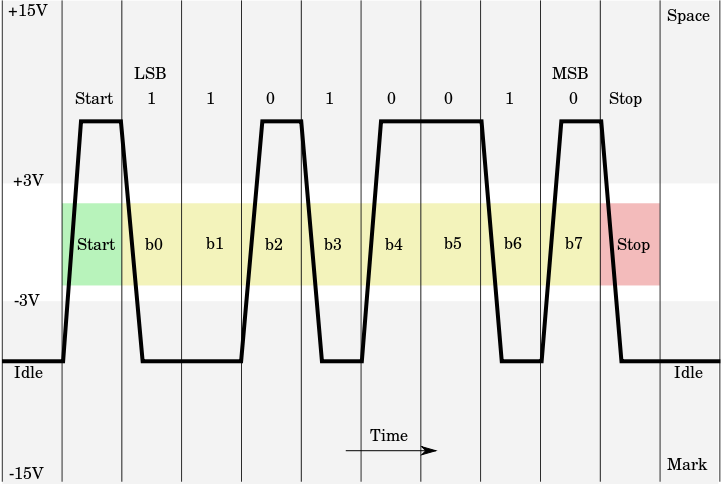
\includegraphics[width=16cm,height=6cm]{UARTprotocol.png}
\caption{UART protocol diagram}
\label{UART protocol diagram}
\end{figure}


UART transmitter controls transmission by fetching a data word in parallel format and directing the UART to transmit it in a serial format. Likewise, the Receiver must detect transmission, receive the data in serial format, strip of the start and stop bits, and store the data word in a parallel format. Since the UART is asynchronous in working, the receiver does not know when the data will come, so receiver generate local clock in order to synchronize to transmitter whenever start bit is received. Asynchronous transmission allows data to be transmitted without the sender having to send a clock signal to the receiver. The transmitter and receiver agree on timing parameters in advance and special bits are added to each word which is used to synchronize the sending and receiving units. When a word is given to the UART for Asynchronous transmission, a bit called the “Start Bit” is added to the beginning of each word that is to be transmitted. The Star Bit is used to alert the receiver that a word of data is about to be sent, and to force the clock in the receiver into synchronization with the clock in the transmitter. After the Start Bit, the individual bits of the word of data are sent, with the Least Significant Bit (LSB) being sent first. Each bit in the transmission is transmitted 
for exactly the same amount of time as all of the other bits, and the receiver “looks” at the wire at approximately halfway through the period assigned to each bit to determine if the bit is a $1$or a $0$. For example, if it takes two seconds to send each bit, the receiver will examine the signal to determine if it is a $1$ or a $0$ after one second has passed, then it will wait two seconds and then examine the value of the next bit, and so on. Then at least one $4$\ Stop Bit is sent by the transmitter. Because asynchronous data is “self-synchronous”, if there is no data to transmit, the transmission line can be idle. \\


\begin{figure}[H]
\centering
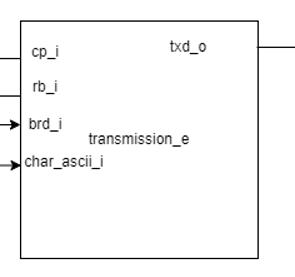
\includegraphics[scale=1.0]{txd.PNG}
\caption{Entity of the transmission block}
\label{Entity of the transmission block}
\end{figure}





\newpage


\raggedright

\newpage                                                                                %biblography
%\section{Reference}
\begin{thebibliography}{}

\bibitem{Intro1}
\texttt{<https://en.wikipedia.org/wiki/Field-programmable\_gate\_array>}

\bibitem{Intro2}
\texttt{<https://www.xilinx.com/products/silicon-devices/fpga/what-is-an-fpga\newline .html>}


\bibitem{Intro3}
\texttt{<https://en.wikipedia.org/wiki/VHDL>}

\bibitem{Intro4}
\texttt{<https://www.101computing.net/wp/wp-content/uploads\\
/morse-code-binary-tree-bg.png>}

\bibitem{Intro5}
\texttt{<https://alpharithms.s3.amazonaws.com/assets/img/ \\
ascii-chart/ascii-table-alpharithms-scaled.jpg>}



\end{thebibliography}



\clearpage

\end{document}
